\documentclass[aspectratio=169, 10pt]{beamer}

\usepackage{bm} % bold math
\usepackage{fontspec}
\usepackage{minted}
\usepackage{pgf-pie}
\usepackage{tikz}

% Custom commands and environments
\makeatletter
\newcommand\version[1]{\renewcommand\@version{#1}}
\newcommand\@version{}
\def\insertversion{\@version}

\newcommand\course[1]{\renewcommand\@course{#1}}
\newcommand\@course{}
\def\insertcourse{\@course}

\newcommand\coursetitle[1]{\renewcommand\@coursetitle{#1}}
\newcommand\@coursetitle{}
\def\insertcoursetitle{\@coursetitle}

\newcommand\lecturenumber[1]{\renewcommand\@lecturenumber{#1}}
\newcommand\@lecturenumber{}
\def\insertlecturenumber{\@lecturenumber}
\makeatother

\newcommand{\slidetitle}[1]{{\xbseries \large \structure{#1}} \bigskip}
\newcommand{\term}[1]{{\color{blue} #1}}
\newcommand{\leftspace}{\hspace{1em}}
\newcommand{\inlinearrow}{
  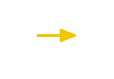
\begin{tikzpicture}[baseline]
    \node [anchor=base] (x) {};
    \draw [rawarrow] (x.mid west) -- ($(x.mid west) + (2em,0)$);
  \end{tikzpicture}
}

\newenvironment{slide}
{\begin{frame}[fragile,environment=slide]\vskip0pt plus 1filll}
{\vskip0pt plus 1filll\end{frame}}

% LaTeX

\setlength{\leftmargini}{1em}

% Common Information

\author{Jon Eyolfson}
\course{ECE 353}
\coursetitle{Systems Software}
\date{2024 Winter}

% fontspec

\defaultfontfeatures{Ligatures=TeX}
% \setmainfont{Domine}
\setsansfont{Inter}[
  FontFace={ul}{n}{Font=*-Thin},
  FontFace={el}{n}{Font=*-ExtraLight},
  FontFace={l}{n}{Font=*-Light},
  FontFace={sb}{n}{Font=*-SemiBold},
  FontFace={eb}{n}{Font=*-ExtraBold},
  FontFace={xb}{n}{Font=*-Black},
]
\setmonofont[Contextuals=AlternateOff, Ligatures=TeXOff]{Iosevka}[
  FontFace={xb}{n}{Font=*-Heavy},
]

%% Font Weights

\DeclareRobustCommand{\ulseries}{\fontseries{ul}\selectfont}
\DeclareTextFontCommand{\textul}{\ulseries}
\DeclareRobustCommand{\elseries}{\fontseries{el}\selectfont}
\DeclareTextFontCommand{\textel}{\elseries}
\DeclareRobustCommand{\lseries}{\fontseries{l}\selectfont}
\DeclareTextFontCommand{\textl}{\lseries}
\DeclareRobustCommand{\sbseries}{\fontseries{sb}\selectfont}
\DeclareTextFontCommand{\textsb}{\sbseries}
\DeclareRobustCommand{\ebseries}{\fontseries{eb}\selectfont}
\DeclareTextFontCommand{\texteb}{\ebseries}
\DeclareRobustCommand{\xbseries}{\fontseries{xb}\selectfont}
\DeclareTextFontCommand{\textxb}{\xbseries}

% tikz

\usetikzlibrary{
  arrows,
  arrows.meta,
  automata,
  backgrounds,
  calc,
  decorations.pathreplacing,
  matrix,
  positioning,
  overlay-beamer-styles,
  shapes,
  shapes.multipart,
  tikzmark,
}

\tikzstyle{rawarrow} = [
  -{Latex[round]},
  line width=1pt,
  yellow,
  shorten >=3pt,
  shorten <=3pt,
  font=\small,
  text=black,
]

\tikzstyle{arrow} = [
  -{Latex[round]},
  line width=1pt,
  yellow,
  shorten >=3pt,
  shorten <=3pt,
  transform canvas={yshift=3pt},
  font=\small,
  text=black,
]

\newcommand{\tikzmarkcoord}[1]{([yshift=3pt]pic cs:#1)}

% minted

\setminted{style=eyolfson, fontsize=\small, escapeinside=||}
\setmintedinline{fontsize=\normalsize}

% hyperref

\hypersetup{colorlinks, urlcolor=blue}

% beamer
\setbeamersize{text margin left=16mm, text margin right=16mm}
\setbeamertemplate{itemize items}[circle]
\setbeamercolor{item}{fg=black}
\setbeamercolor{structure}{fg=darkblue}
\setbeamerfont{frametitle}{series=\bfseries, parent=structure}
\setbeamertemplate{navigation symbols}{}
\setbeamertemplate{headline}{}
\setbeamertemplate{footline}{
  \begin{tikzpicture}[
    remember picture,
    overlay,
    shift={(current page.south west)},
  ]
    \path [fill=gray] (144mm, 0) -- (160mm, 16mm) -- (160mm, 0);
    \node [inner sep=3.5mm, outer sep=0, text=black, anchor=base east,
           align=right, yshift=3.5mm]
          at (current page.south east) {\ttfamily \small \insertframenumber{}};
  \end{tikzpicture}
}
\setbeamertemplate{title page}{
  \begin{tikzpicture}[
    remember picture,
    overlay,
    shift={(current page.south west)},
    background rectangle/.style={fill=darkblue},
    show background rectangle,
  ]
    \node [anchor=center, align=center, text=white, text width=40mm, scale=3.2]
          at (\paperwidth / 2, \paperheight * 2 / 3)
          {\xbseries \inserttitle{}};
    \node [anchor=base west, align=left, inner sep=0, text=white, yshift=2.5mm]
          at (16mm, \paperheight / 3)
          {\insertdate{} \insertcourse{}: \insertcoursetitle{}};
    \node [anchor=base west, align=left, inner sep=0, text=white, yshift=-2.5mm]
          at (16mm, \paperheight / 3)
          {\insertauthor};
    \node [anchor=base east, align=right, inner sep=0, text=white, yshift=2.5mm]
          at (144mm, \paperheight / 3)
          {Lecture \insertlecturenumber{}};
    \node [anchor=base east, align=right, inner sep=0, text=white,
           yshift=-2.5mm]
          at (144mm, \paperheight / 3)
          {\ttfamily \insertversion{}};
    \node [align=center, anchor=south, inner sep=0, text=white, yshift=3.5mm]
          (license) at (\paperwidth / 2, 0)
          {\fontsize{7pt}{7pt}\selectfont This  work is licensed under a
           \href{http://creativecommons.org/licenses/by-sa/4.0/}
                {\color{lightblue} Creative Commons Attribution-ShareAlike 4.0
                 International License}};
  \end{tikzpicture}
}

% xcolor

%% Primary Colour

\definecolor{pantone655}{RGB}{0, 42, 92} % #002a5c
\colorlet{darkblue}{pantone655}

%% Secondary Colours

\definecolor{pantone633}{RGB}{0, 139, 176} % #008bb0
\colorlet{blue}{pantone633}

\definecolor{pantonewarmred}{RGB}{220, 70, 51} % #dc4633
\colorlet{red}{pantonewarmred}

\definecolor{pantone3285}{RGB}{0, 161, 137} % #00a189
\colorlet{cyan}{pantone3285}

\definecolor{pantone7722}{RGB}{13, 83, 77} % #0d534d
\colorlet{darkcyan}{pantone7722}

\definecolor{pantone376}{RGB}{141, 191, 46} % #8dbf2e
\colorlet{green}{pantone376}

\definecolor{pantone2613}{RGB}{109, 36, 122} % #6d247a
\colorlet{violet}{pantone2613}

\definecolor{pantone2985}{RGB}{111, 199, 234} % #6fc7ea
\colorlet{lightblue}{pantone2985}

\definecolor{pantone227}{RGB}{171, 19, 104} % #ab1368
\colorlet{magenta}{pantone227}

\definecolor{pantone7406}{RGB}{241, 197, 0} % #f1c500
\colorlet{yellow}{pantone7406}

%% Neutrals

\definecolor{pantonecoolgray2}{RGB}{208, 209, 201} % #d0d1c9
\colorlet{gray}{pantonecoolgray2}


\lecturenumber{1}
\title{Why Operating\\Systems?}
\version{2.0.1}

\begin{document}

\begin{frame}[plain, noframenumbering]
  \titlepage
\end{frame}

\begin{slide}

  \slidetitle{I'm Jon, Your Instructor}

  \centering
  
\begin{tikzpicture}[every node/.style={anchor=base, align=center}]
    \node [visible on=<1>] (eyolfson) {\bfseries \Huge Eyolfson};
    \node [visible on=<2>] {\bfseries \Huge \color{red} Eyolfson};
    \node [visible on=<3-4>, anchor=base west] at (eyolfson.base west)
          {\bfseries \Huge Elf};
    \node [visible on=<4>, anchor=base east] at (eyolfson.base east)
          {\bfseries \Huge son};
    \node [visible on=<5>, anchor=base west] at (eyolfson.base west)
          {\bfseries \Huge E};
    \node [visible on=<5>, anchor=base east] at (eyolfson.base east)
          {\bfseries \Huge lfson};
    \node [visible on=<6>] {\bfseries \Huge E{\color{blue}yo}lfson};
  \end{tikzpicture}

\end{slide}

\begin{slide}
  
  \slidetitle{Why Operating Systems?}
  
  Understanding the operating system will make you a better programmer
  \bigskip

  You will either write software that:
  \begin{itemize}
    \item Interacts with the operating system
    \item Is the operating system
  \end{itemize}
\end{slide}

\begin{slide}
  
  \slidetitle{Important URLs for Course Resources}

  Public: \url{https://eyolfson.com/}
  \medskip

  Private: \url{https://q.utoronto.ca/} (Quercus)
\end{slide}

\begin{slide}
  
  \slidetitle{Labs on GitLab, Discussion on Discord, Streams on YouTube}

  \begin{center}
    
\includegraphics[width=64mm]{gitlab.eps}
    \bigskip

    
\includegraphics[width=64mm]{discord.eps}
    \bigskip

    
\includegraphics[width=64mm]{youtube.eps}
  \end{center}

  Sign in: \url{https://compeng.gg/discord/join/ece353/}
\end{slide}

\begin{slide}
  
  \slidetitle{Lecture Attendance is Still Important}

  It's much faster to get feedback from you and clarify if anything is unclear
  \medskip

  We'll have live coding, I'll be able to explain any happy accidents
  \medskip

  If there's anything else I can do to make attending a better experience
  
  let me know!
\end{slide}

\begin{slide}
  
  \slidetitle{Evaluation for this Course}

  \centering
  \begin{tabular}{lll}
      \textbf{Assessment} & \textbf{Weight} & \textbf{Due Date} \\
      Lab 0 & 1\% & January 18 \\
      Lab 1 & 4\% & January 25 \\
      Lab 2 & 4\% & February 8 \\
      Midterm Exam & 25\% & February 26 @ 6:30 PM \\
      Lab 3 & 4\% & February 29 \\
      Lab 4 & 4\% & March 14 \\
      Lab 5 & 4\% & March 28 \\
      Lab 6 & 4\% & April 11 \\
      Final Exam & 50\% & April 16 to April 30 \\
  \end{tabular}
\end{slide}

\begin{slide}
  
  \slidetitle{Academic Honesty Policy}

  You can study together, discuss concepts on Discord
  \medskip

  Don't post lab code on Discord, any other code is okay
  \medskip

  Any cheating is not tolerated, and will only hurt you
\end{slide}

\begin{slide}
  
    \slidetitle{The Recommended Books Complement Lectures}

    ``\href{https://pages.cs.wisc.edu/~remzi/OSTEP/}
           {Operating Systems: Three Easy Pieces}'' \\
    by \href{http://www.cs.wisc.edu/~remzi/}{Remzi Arpaci-Dusseau}
    and \href{http://www.cs.wisc.edu/~dusseau/}{Andrea Arpaci-Dusseau}
    \bigskip

    ``\href{https://en.wikipedia.org/wiki/The_C_Programming_Language}
           {The C Programming Language}'' \\
    by \href{https://en.wikipedia.org/wiki/Brian_Kernighan}{Brian Kernighan}
    and \href{https://en.wikipedia.org/wiki/Dennis_Ritchie}{Dennis Ritchie}
\end{slide}

\begin{slide}
  
  \slidetitle{Skills You Should Practice Again If Needed}

  C programming and debugging
  \medskip

  Being able to convert between binary, hex, and decimal
  \medskip

  Little-endian and big-endian
  \medskip

  Memory being byte-addressable, memory addresses (pointers)
\end{slide}

\begin{slide}
  
  \slidetitle{Please Provide Feedback!}

  This course is challenging, please let me know if anything is unclear
  \medskip

  You can ask interesting questions, all programs interact with the OS
  \medskip

  By the end of the course you'll be a better programmer
\end{slide}

\begin{slide}
  
  \slidetitle{An Operating System Manages Resources}

  \centering

  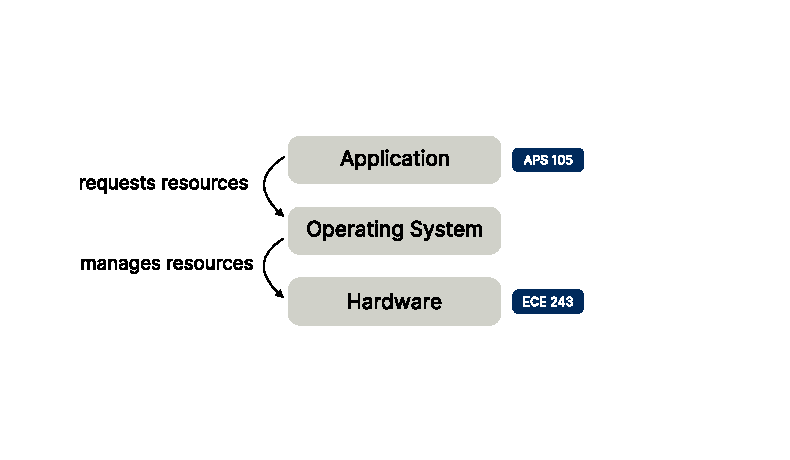
\includegraphics{operating-system-overview.eps}

\end{slide}

\begin{slide}
  
  \slidetitle{There's 3 Core Operating System Concepts}

  \textbf{Virtualization:} share one resource by mimicking
  
  \leftspace{}multiple independent copies
  \bigskip

  \textbf{Concurrency:} handle multiple things happening at the same time
  \bigskip

  \textbf{Persistence:} retain data consistency even without power
\end{slide}

\begin{slide}

  ``All problems in computer science can be solved by another level of
  indirection''

  \begin{flushright}
    - David Wheeler
  \end{flushright}

\end{slide}

\begin{slide}
  
  \slidetitle{Our First Abstraction is a Process}

  \textbf{Program:} a file containing all the instructions and data required
  to run
  \bigskip

  \textbf{Process:} an instance of running a program
\end{slide}

\begin{slide}
  
  \slidetitle{The Basic Requirements for a Process}

  \centering
  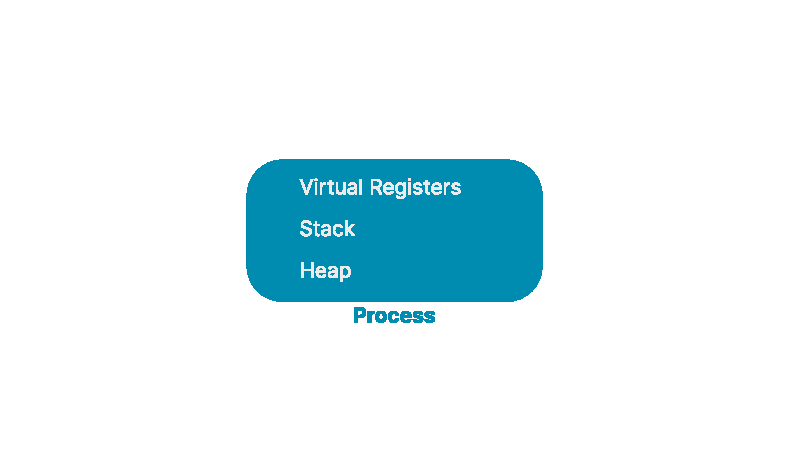
\includegraphics{process-basic.eps}

\end{slide}

\begin{slide}
  
  \slidetitle{My First Question to You}

  How are you able to run two different programs at the same time?
  \medskip

  For example, a ``hello world'' program and another that
  
  \leftspace{}counts up one every second
\end{slide}

\begin{slide}
  
  \slidetitle{Does the OS Allocate Different Stacks For Each Process?}

  The stacks for each process need to be in physical memory
  \medskip

  One option is the operating system just allocates
  
  \leftspace{}any unused memory for the stack
  \medskip

  Would there be any issues with this?
\end{slide}

\begin{slide}
  
  \slidetitle{What About Global Variables?}

  The compiler needs to pick an address for each variable when you compile
  \medskip

  What if we had a global registry of addresses?
  \medskip

  Would there be any issues with this?
\end{slide}

\begin{slide}
  
  \slidetitle{Potential Memory Layout for Multiple Processes}

  \centering

  \includegraphics<1>{memory-layout-first.eps}%
  \includegraphics<2>{memory-layout-second.eps}
\end{slide}

\begin{slide}
  
  \slidetitle{What Happens If Two Processes Run the Same Program?}

  \inputminted{c}{count.c}

\end{slide}

\begin{slide}
  
  \slidetitle{What Did We Find?}

  Was the address of \mintinline{c}{local} the same between the two processes?
  \medskip

  Was the address of \mintinline{c}{global} the same between the two processes?
  \medskip

  What else may be needed for a process?
\end{slide}

\begin{slide}
  
  \slidetitle{A Process Has Its Own Virtual Memory}

  \centering

  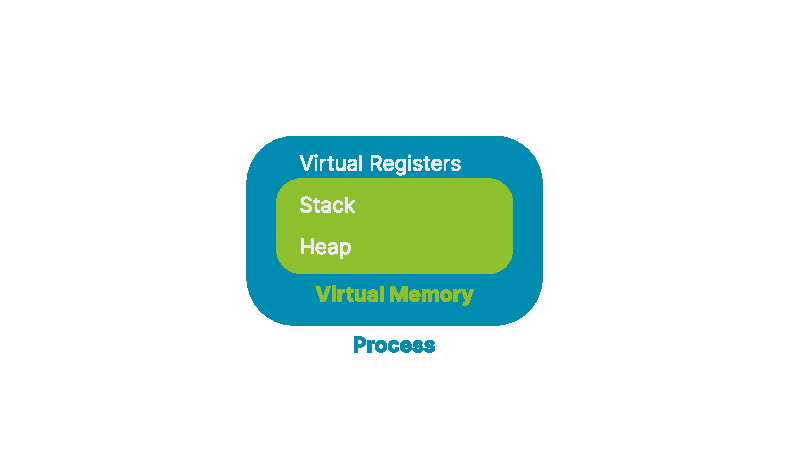
\includegraphics{process-virtual-memory.eps}

\end{slide}

\begin{slide}
  
  \slidetitle{Example Code from This Class}

  All code will be in the ``materials'' repository located:

  \url{https://laforge.eecg.utoronto.ca/ece353/2024-winter/student/materials/}
  \bigskip

  Compile the code:
  \begin{minted}{bash}
cd lectures/01-why-operating-systems
meson setup build
meson compile -C build
  \end{minted}
  \bigskip

  Execute the code:
  \begin{minted}{bash}
build/read-four-bytes <FILE>
  \end{minted}
  \bigskip

  Source:
  \href{https://laforge.eecg.utoronto.ca/ece353/2024-winter/student/materials/-/blob/main/lectures/01-why-operating-systems/read-four-bytes.c}
       {\ttfamily materials/lectures/01-why-operating-systems/read-four-bytes.c}
\end{slide}

\begin{slide}

  \slidetitle{Believe It or Not, This Is ``Hello world''}

  \small \ttfamily
  0x7F 0x45 0x4C 0x46 0x02 0x01 0x01 0x00 0x00 0x00 0x00 0x00 0x00 0x00 0x00
  0x00 \newline
  0x02 0x00 0xB7 0x00 0x01 0x00 0x00 0x00 0x78 0x00 0x01 0x00 0x00 0x00 0x00
  0x00 \newline
  0x40 0x00 0x00 0x00 0x00 0x00 0x00 0x00 0x00 0x00 0x00 0x00 0x00 0x00 0x00
  0x00 \newline
  0x00 0x00 0x00 0x00 0x40 0x00 0x38 0x00 0x01 0x00 0x40 0x00 0x00 0x00 0x00
  0x00 \newline
  0x01 0x00 0x00 0x00 0x05 0x00 0x00 0x00 0x00 0x00 0x00 0x00 0x00 0x00 0x00
  0x00 \newline
  0x00 0x00 0x01 0x00 0x00 0x00 0x00 0x00 0x00 0x00 0x01 0x00 0x00 0x00 0x00
  0x00 \newline
  0xA8 0x00 0x00 0x00 0x00 0x00 0x00 0x00 0xA8 0x00 0x00 0x00 0x00 0x00 0x00
  0x00 \newline
  0x00 0x10 0x00 0x00 0x00 0x00 0x00 0x00 0x08 0x08 0x80 0xD2 0x20 0x00 0x80
  0xD2 \newline
  0x81 0x13 0x80 0xD2 0x21 0x00 0xA0 0xF2 0x82 0x01 0x80 0xD2 0x01 0x00 0x00
  0xD4 \newline
  0xC8 0x0B 0x80 0xD2 0x00 0x00 0x80 0xD2 0x01 0x00 0x00 0xD4 0x48 0x65 0x6C
  0x6C \newline
  0x6F 0x20 0x77 0x6F 0x72 0x6C 0x64 0x0A
\end{slide}

\end{document}